% Set spellcheck for TexStudio
%!TeX spellcheck = en_US
%!TeX root = ../thesis.tex


\chapter{Conclusion}
Here are the results of the performance benchmarking summarized and conclusions stated that answer the research questions proposed in Chapter \ref{sec:methodology}. The first concern is, if there are regimes where the newly proposed algorithms perform faster than a Allreduce or Allgather implementation that only use a dense or sparse representation of the sets respectively. For this the run times of the newly proposed \texttt{Union\_Butterfly} is compared against its analog Allreduce and Allgather in Figure \ref{fig:exampleConculsion} as an example. The benchmark was done using $p=(32\times32)$ processors.
\begin{figure}[h]
	\centering
	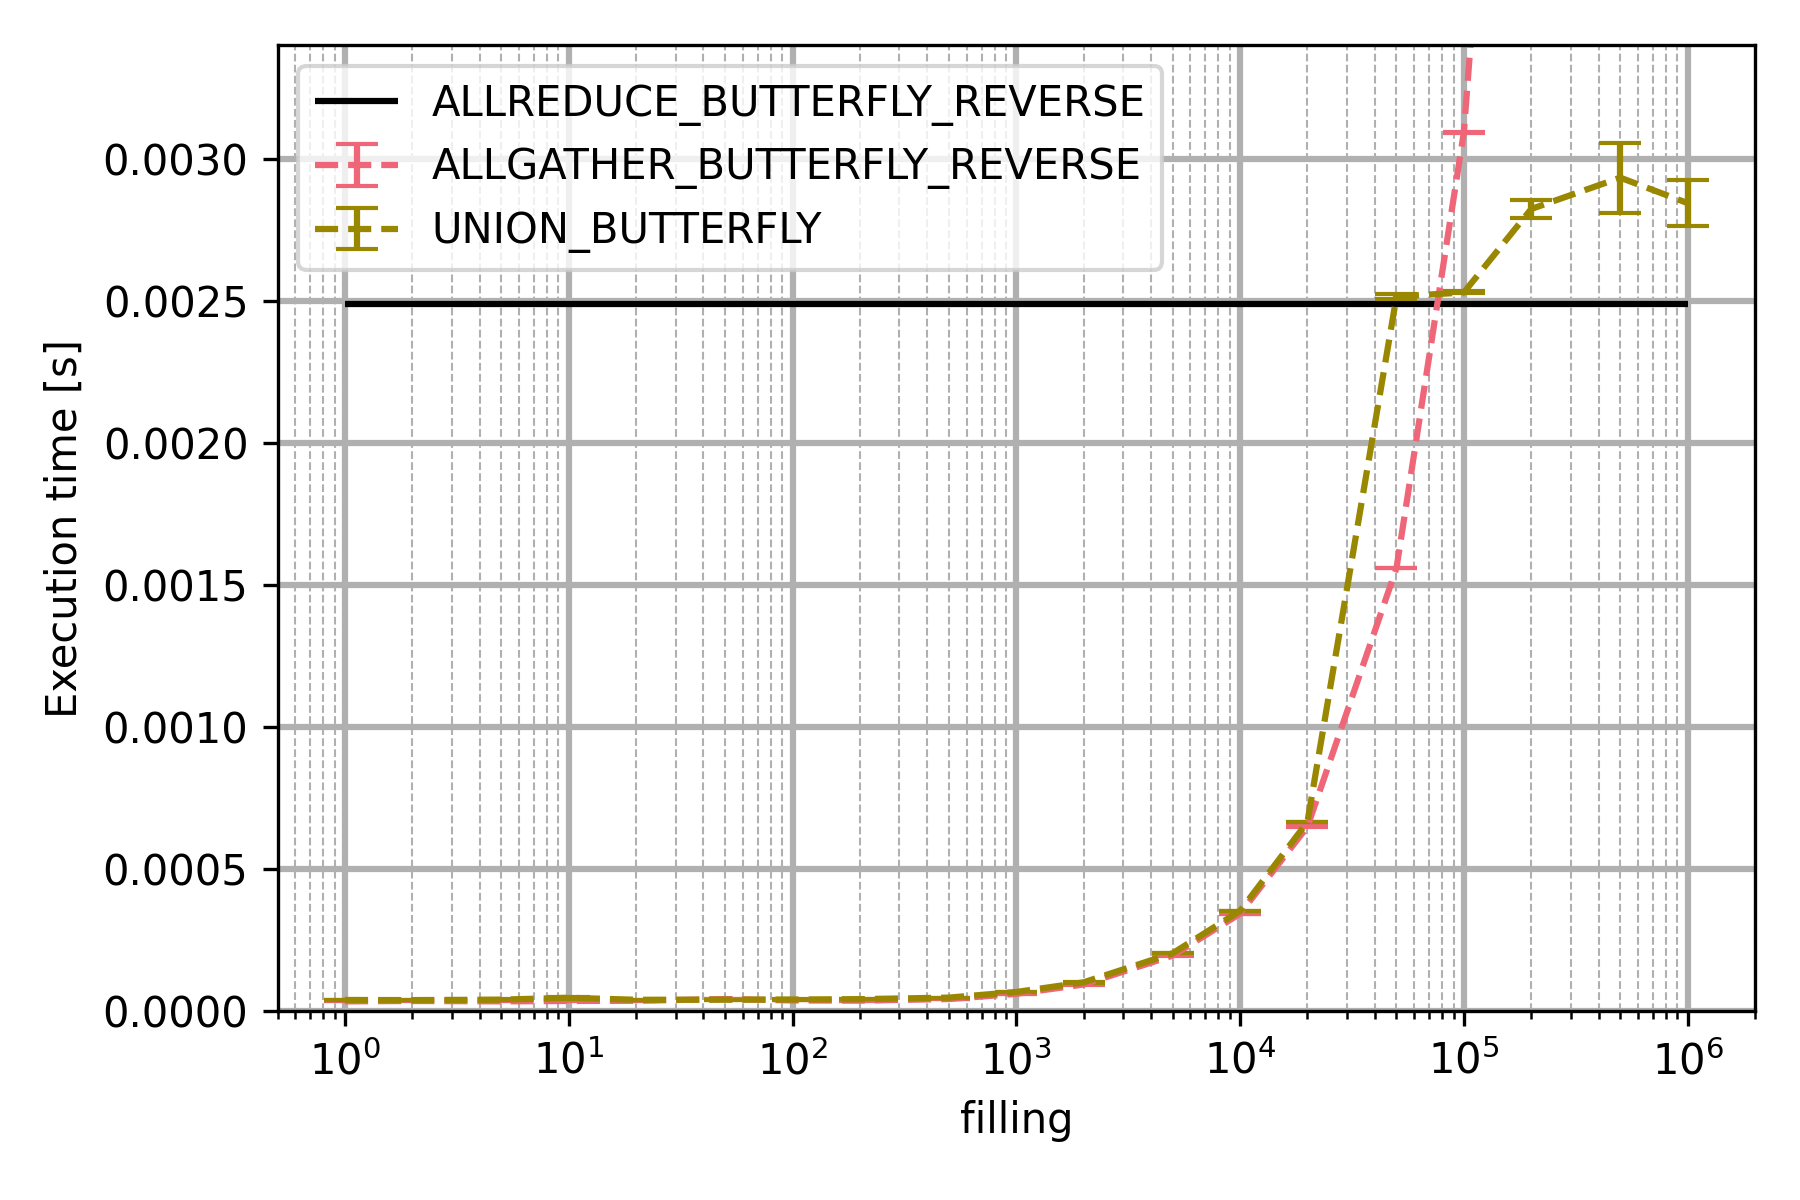
\includegraphics[width=0.7\textwidth]{../plots/ExampleConclusion/32x32ExampleConclusion.png}
	\caption{Execution time of the algorithms \texttt{Allreduce\_Butterfly\_Reverse}, \texttt{Allgather\_Butterfly\_Reverse} and \texttt{Union\_Butterfly} against the set filling. The set size is $10^7$ elements.}
	\label{fig:exampleConculsion}
\end{figure}
Here it is apparent that there are indeed configurations where the new Union algorithm is faster than either the Allgather or the Allreduce. In fact one can see that for set fillings below $5\cdot10^4$ the run time of \texttt{Union\_Butterfly} orients itself on the run time of the Allgather and is therefore faster than the Allreduce. For set fillings higher than this threshold the execution time is more or less proportional to the one of the Allreduce and is therefore faster than the Allgather. In this setup one can therefore model the run time as 
\begin{align*}
	T_\mathrm{Union} \leq c \cdot \min(T_\mathrm{Allreduce}, T_\mathrm{Allgather}).
\end{align*}
The constant $c$ is in all setups greater than 1. The most relevant filling regime is for high fillings as here the execution time is already the highest so even small relative changes can have a big impact on the runtime of an algorithm where the Union operations are used. In the case shown in Figure \ref{fig:exampleConculsion} \texttt{Union\_Butterfly} is around 12\% slower than the Allreduce. This is not true for every setup.\\
Especially, if only one process per node is used the new union algorithms are up to 2 times slower than their foundation Allreduce. A usage for this application is therefore not recommended. For the processor layouts using every processor there are also restrictions where good performance is expected. Firstly if the number of processors is a power of two \texttt{Union\_Butterfly} is always faster than \texttt{Union\_Shift}. \texttt{Union\_Butterfly} performs well for set sizes over $5\cdot10^5$ and is here only a few percent slower than its foundation Allreduce in the worst case. For \texttt{Union\_Shift} this threshold lies in the order of $10^7$ elements. The foundation Allreduce implementations are generally slower than the best performing native Allreduce provided by an optimized MPI library. This could be due to worse implementation in C or to the fact that other Allreduce algorithms perform faster in the tested regime. In the proposed regimes for the set sizes the foundation algorithms can be up to 30\% slower than the library variant, but can also be as fast or in some cases faster.\\ 
Considering the case where the sets are sparsely filled and only the sparse representation is used, the used foundation Allgather implementations are faster or as fast as the reference Allgather provided by the MPI library. Also for the final union algorithms are no significant slow downs apparent that could have an important influence on the performance. It matters how the distribution of set fillings over the processors is. If the sets are uniformly filled the implementations are faster than if only one process holds all elements. This is true for all tested implementations.\\
Our newly proposed algorithms have both a tunable parameter '$critSize$'. This parameter defines the threshold of set filling when a process switches from the sparse representation to the dense one. Obviously it was found that for small values the execution time of the adaptive union algorithms tend to look earlier (for smaller set fillings) like the reference Allreduce implementation. For larger values of '$critSize$' the run time of the adaptive union algorithms follow the trend of the Allgather for longer. The parameter '$critSize$' has also an influence for total set fillings that are slightly greater than itself as the switching of representation happens during the execution of the union algorithms. This can lead to an overshoot of execution time if '$critSize$' is tuned to be the memory footprint where the dense representation is smaller. This results in a trade-off situation as this overshoot in run time is not wanted and on the other hand it is favorable to keep the execution time as long as possible close to the Allgather run time complexity. As a good value that brings balanced results is 
\begin{align*}
	critSize = \frac{p-1}{32p\log(p)}|\Tilde{S}|,
\end{align*}
where $p$ is the number of processors and $|\Tilde{S}|$ the size of the underlying set.\\
As the motivation for these adaptive union set operation algorithms is using them for a BFS implementation \texttt{Union\_Butterfly} and \texttt{Union\_Shift} where tested for this use case. Here it is apparent that implementations using the new union algorithms are for the most cases indeed faster than an implementation using the fastest available Allreduce implementation. For a power of two number of processors \texttt{Union\_Butterfly} is again the fastest one. 
The algorithms perform relatively better for graphs with larger number of vertices as they correspond in this case to the underlying set. So positive performance effects are seen on graphs with more than $10^5$ vertices. The strength of the new union implementations can be seen, if the topology of the graphs is quite long (i.e. for graphs with great diameter). There are also huge performance gains for graphs that are disjoint. Both of these cases are expected to be beneficial as here the sparse variant is used more often than in a uniform connected graph.

\section{Future Work}
This thesis leads to new open questions and ideas that can be explored. Firstly the analysis of the parameter $critSize$ can be done more thoroughly. Here is only a rule of thumb value found that worked sufficiently well. There can be even strategies applied that this parameter is not constant in each iteration of the algorithms. This may can lead to a better trade-off of overshooting run time.\\
Another idea that can be implemented is the usage of a super dense sparse format. The sets can also be represent by a list of elements that are missing compared to the underlying set $\Tilde{S}$. For very large set fillings this representation could be more efficient than the dense bitmap representation. Of corse here two lists in this format can not be combined into a single one by simply appending them as this would not perform a union operation. Also one needs to keep an overview how many bits are set in the dense bitmap to get information when to switch to the super dense representation. Therefore more computation would be needed, but there could be still overall performance gains visible.\\
This idea leads to the idea of extending the family of adaptive set operation algorithms to also support an intersection operation. For the intersection the algorithm can be equivalently build but using the super dense sparse representation instead of the normal sparse one. This works as the concatenation of two lists that contain the elements that are not in the sets correspond to the intersection of these sets.\\
There also needs to be consideration done, if an implementation for the symmetric difference (performing a exclusive OR over set elements) can be done. The problem is here that the number of elements does not rise or fall monotonically if it is applied over multiple sets. Therefore a bookkeeping of the number of set elements is mandatory no matter which sparse representation is used as adaptation.\\
The family of adaptive set operation algorithms can also be extended to work optimally for smaller set sizes. In this thesis the foundation Allreduce was chosen to be build out of a Reducescatter and an Allgather phase. This works optimally for large set sizes. There are also algorithms that are expected to perform better for smaller message sizes. These algorithms typically need less iterations, but instead send the whole message array. Using a sparse format could have a bigger impact as the relative message size gain would be greater. Especially when considering using only 16-bit integer for set sizes below 65536. The trade-off is here of course that computational overhead is more relevant, if the message sizes are small. 















